\documentclass[10pt,twocolumn,a4paper]{article}

\usepackage[margin=1.8cm]{geometry}
\usepackage{graphicx}
\usepackage{amsmath}
\usepackage{amssymb}
\usepackage{booktabs}
\usepackage{hyperref}

\title{\textbf{Logarithmic Oscillatory Dark Energy: Empirical Fit to Pantheon+ SNe Ia and Predictive Turnaround Forecasts for the ESA Euclid Space Telescope}}

\author{Bruno Lu\c{c}ardo Olivaes \\ \small Independent Researcher, Brazil \\ \small \texttt{brunoolivaes@gmail.com}}

\date{\today}

\begin{document}

\twocolumn[{%
  \begin{@twocolumnfalse}
    \maketitle
    \begin{abstract}
    \noindent Standard Chevallier-Polarski-Linder (CPL) dark energy parameterizations ($w(a) = w_0 + w_a(1-a)$) indicate an escalating phantom behavior ($w < -1$) at intermediate redshifts, but diverge uncontrollably into unphysical regimes as $z \to \infty$. Here, we formulate a bounded, harmonic parameterization of dynamical dark energy governed by scale-invariant logarithmic oscillation in cosmic scale factor $a$: $w(a) = -1 + A \sin\left(\frac{2\pi}{\lambda}\ln(a) + \phi_0\right)$. By integrating the relativistic fluid continuity equation, we derive the exact closed-form expression for the dark energy density $\rho_{\mathrm{DE}}(z)$. We calibrate this phenomenological framework against 1,590 Type Ia Supernovae from the Pantheon+ compilation ($z \in [0.01, 2.26]$). The oscillatory framework achieves an optimal minimum with $H_0 = 71.08\text{ km/s/Mpc}$, $\Omega_m = 0.355$, and $\chi^2 = 772.59$, delivering an empirical fit comparable to DESI CPL ($\Delta\chi^2 = -10.86$, $\Delta\mathrm{AIC} = -4.86$). Evaluating model selection criteria, we find that while the Akaike criterion supports the dynamical fit, the Bayesian Information Criterion penalizes the three additional parameters ($\Delta\mathrm{BIC} = +11.25$), demonstrating that current supernova datasets alone cannot definitively break the Occam's razor degeneracy. Crucially, we show that upcoming high-redshift observations from the ESA Euclid Space Telescope at $z \in [1.5, 3.0]$ possess the discriminatory power required: while linear CPL monotonically plunges to $w(z=3) = -2.04$, the oscillatory model predicts a distinctive turnaround toward non-phantom values ($w(z=3) = -1.60$), yielding a decisive testable separation of $\Delta w = +0.44$.
    \end{abstract}
    \vspace{0.6cm}
  \end{@twocolumnfalse}
}]

\section{Introduction}
The persistent tension between early-universe determinations of the Hubble constant from Planck cosmic microwave background observations ($H_0 \approx 67.4\text{ km/s/Mpc}$) and local distance ladder measurements from the SH0ES collaboration ($H_0 \approx 73.0\text{ km/s/Mpc}$) suggests that the standard spatially flat $\Lambda\mathrm{CDM}$ cosmological model may be incomplete. In parallel, recent baryon acoustic oscillation (BAO) measurements from the Dark Energy Spectroscopic Instrument (DESI) Year 1 data release, combined with CMB and Type Ia supernovae (SNe Ia), have highlighted empirical indications of dynamical dark energy ($w(z) \neq -1$) at $2.6\sigma$ to $3.9\sigma$ significance \cite{desi2024}.

In standard observational analyses, dynamical dark energy is commonly parameterized via the linear Chevallier-Polarski-Linder (CPL) expansion \cite{chevallier2001,linder2003}:
\begin{equation}
w_{\mathrm{CPL}}(a) = w_0 + w_a(1-a) = w_0 + w_a\frac{z}{1+z}.
\label{eq:cpl}
\end{equation}
While linear CPL is analytically straightforward in the low-redshift regime ($z \ll 1$), it represents a truncated first-order Taylor expansion around the present epoch ($a=1$). Consequently, when extrapolated to high redshifts ($z \ge 2$), it predicts monotonic divergence into deep phantom regimes ($w \to -\infty$ as $z \to \infty$), presenting theoretical challenges related to phantom singularities and vacuum stability.

In this work, we investigate a bounded alternative: logarithmic oscillatory dark energy. Logarithmic periodicities naturally arise in physical contexts characterized by scale invariance, axion monodromy potentials, cyclic cosmological models, and higher-dimensional bulk leakage. We obtain the exact analytical solution for $\rho_{\mathrm{DE}}(z)$, evaluate the model against the Pantheon+ SNe Ia compilation, perform a transparent information-criterion audit ($\Delta\mathrm{AIC}$ and $\Delta\mathrm{BIC}$), and present sharp, falsifiable predictions for upcoming wide-field surveys with the ESA Euclid and NASA Nancy Grace Roman space telescopes.

\section{Model Formulation and Exact Analytical Solution}
Consider a flat Friedmann-Lema\^{i}tre-Robertson-Walker (FLRW) universe. We define the effective dark energy equation of state via a logarithmic harmonic oscillation:
\begin{equation}
w(a) = -1 + A \sin\left(\frac{2\pi}{\lambda}\ln(a) + \phi_0\right),
\label{eq:w_osc}
\end{equation}
where $A$ is the dimensionless amplitude, $\lambda$ is the logarithmic wavelength period, and $\phi_0$ is the present-day phase. Unlike linear expansions, $w(a)$ remains strictly bounded within the physical envelope $[-1-A, -1+A]$ across all cosmological epochs $a \in (0, 1]$.

\subsection{Theoretical Context and the Phantom Divide}
We treat Eq.~\eqref{eq:w_osc} as a phenomenological kinematic ansatz for the effective dark energy evolution. In canonical single-field quintessence models with standard kinetic terms, crossing the phantom divide ($w = -1$) is mathematically prohibited by the null energy condition, and naive transitions trigger ghost instabilities. However, within the framework of Effective Field Theories (EFT) of dark energy, ghost-free crossings of $w = -1$ are well-established in models featuring non-canonical kinetic terms ($k$-essence), Galileon/Horndeski scalar-tensor couplings, or multi-field configurations with negative metric signatures \cite{vikman2005,hu2005,creminelli2009}. In this context, Eq.~\eqref{eq:w_osc} represents an effective low-energy description of these rich dynamical sectors.

\subsection{Exact Continuity Integration}
The cosmological evolution of the dark energy density $\rho_{\mathrm{DE}}(a)$ is governed by the relativistic continuity equation:
\begin{equation}
\frac{d\ln\rho_{\mathrm{DE}}}{d\ln a} = -3\left[1 + w(a)\right] = -3 A \sin\left(\frac{2\pi}{\lambda}\ln a + \phi_0\right).
\label{eq:continuity}
\end{equation}
Integrating Eq.~\eqref{eq:continuity} from the present epoch ($a=1$, where $\ln a = 0$) to an arbitrary scale factor $a = (1+z)^{-1}$ gives:
\begin{equation}
\ln\left(\frac{\rho_{\mathrm{DE}}(a)}{\rho_0}\right) = -3 A \int_{0}^{\ln a} \sin\left(\frac{2\pi}{\lambda} u + \phi_0\right) du.
\label{eq:integral}
\end{equation}
Evaluating this definite integral analytically yields:
\begin{align}
\int_{0}^{\ln a} & \sin\left(\frac{2\pi}{\lambda} u + \phi_0\right) du \nonumber \\
&= \left[ -\frac{\lambda}{2\pi} \cos\left(\frac{2\pi}{\lambda}u + \phi_0\right) \right]_{0}^{\ln a} \nonumber \\
&= \frac{\lambda}{2\pi} \left[ \cos\phi_0 - \cos\left(\frac{2\pi}{\lambda}\ln a + \phi_0\right) \right].
\end{align}
Substituting this closed form back into Eq.~\eqref{eq:integral}, we obtain the exact analytical dark energy density:
\begin{equation}
\begin{split}
\frac{\rho_{\mathrm{DE}}(z)}{\rho_0} = \exp\Bigg( &-\frac{3 A \lambda}{2\pi} \Big[ \cos\phi_0 \\
&- \cos\left(-\frac{2\pi}{\lambda}\ln(1+z) + \phi_0\right) \Big] \Bigg).
\end{split}
\label{eq:rho_exact}
\end{equation}
The Hubble parameter $H(z)$ for a flat universe with matter density $\Omega_m$ and dark energy density $\Omega_{\mathrm{DE}} = 1 - \Omega_m$ is given analytically by:
\begin{equation}
H(z) = H_0 \left[ \Omega_m (1+z)^3 + (1-\Omega_m) \frac{\rho_{\mathrm{DE}}(z)}{\rho_0} \right]^{1/2}.
\label{eq:hubble}
\end{equation}

\section{Observational Calibration: Pantheon+ SNe Ia}
We calibrated the model against the Pantheon+ sample of 1,590 spectroscopically confirmed Type Ia Supernovae across $0.001 < z < 2.26$ \cite{brout2022}. The theoretical distance modulus is:
\begin{equation}
\mu_{\mathrm{theo}}(z) = 5\log_{10}\left(\frac{d_L(z)}{10\text{ pc}}\right),
\end{equation}
where $d_L(z) = (1+z) c \int_0^z \frac{dz'}{H(z')}$. Model parameters were determined by minimizing:
\begin{equation}
\chi^2 = \sum_{i=1}^{1590} \frac{\left[\mu_{\mathrm{obs}, i} - \mu_{\mathrm{theo}}(z_i)\right]^2}{\sigma_i^2}.
\end{equation}

To rigorously evaluate whether the empirical fit justifies the additional parameters, we compute both the Akaike Information Criterion ($\mathrm{AIC} = \chi^2 + 2k$) and the Bayesian Information Criterion ($\mathrm{BIC} = \chi^2 + k\ln N$), where $k$ is the number of free parameters and $N = 1,590$:

\begin{table}[h]
\centering
\caption{Cosmological best-fit parameters and information criteria across 1,590 Pantheon+ SNe Ia.}
\label{tab:fits}
\resizebox{\columnwidth}{!}{%
\begin{tabular}{lccccccr}
\toprule
Model & $k$ & $H_0$ & $\Omega_m$ & $\chi^2$ & $\Delta\chi^2$ & $\Delta\mathrm{AIC}$ & $\Delta\mathrm{BIC}$ \\
\midrule
$\Lambda\mathrm{CDM}$ & 2 & 71.81 & 0.413 & 783.45 & Ref. & Ref. & Ref. \\
DESI CPL & 4 & 71.06 & 0.339 & 772.29 & $-11.16$ & $-7.16$ & $+3.58$ \\
\textbf{Log-Osc.} & \textbf{5} & \textbf{71.08} & \textbf{0.355} & \textbf{772.59} & \textbf{$-10.86$} & \textbf{$-4.86$} & \textbf{$+11.25$} \\
\bottomrule
\end{tabular}%
}
\end{table}

\subsection{Information-Theoretic Model Selection}
Table~\ref{tab:fits} reveals a vital methodological distinction:
\begin{enumerate}
\item In terms of raw goodness-of-fit, both dynamical dark energy formulations achieve an almost identical, significant $\chi^2$ reduction of $\Delta\chi^2 \approx -11$ relative to $\Lambda\mathrm{CDM}$.
\item Under the Akaike criterion, both models are preferred over $\Lambda\mathrm{CDM}$ ($\Delta\mathrm{AIC} = -7.16$ for CPL and $-4.86$ for Log-Oscillatory), indicating that the dynamical degrees of freedom capture genuine variance in the expansion history.
\item Crucially, under the Bayesian Information Criterion, the large sample size ($N = 1,590$, $\ln N \approx 7.37$) imposes a stringent Occam's razor penalty for additional free parameters ($\Delta k = 3$). This results in $\Delta\mathrm{BIC} = +11.25$. In Bayesian statistics, $\Delta\mathrm{BIC} > +10$ constitutes strong evidence favoring the parsimony of flat $\Lambda\mathrm{CDM}$ when supernova data is evaluated in isolation.
\end{enumerate}
This finding illustrates a central reality of modern observational cosmology: current low-to-intermediate redshift distance-ladder probes cannot definitively distinguish dynamical dark energy from statistical overfitting. This statistical impasse provides the exact scientific imperative for high-redshift geometric measurements.

\begin{figure}[t]
\centering
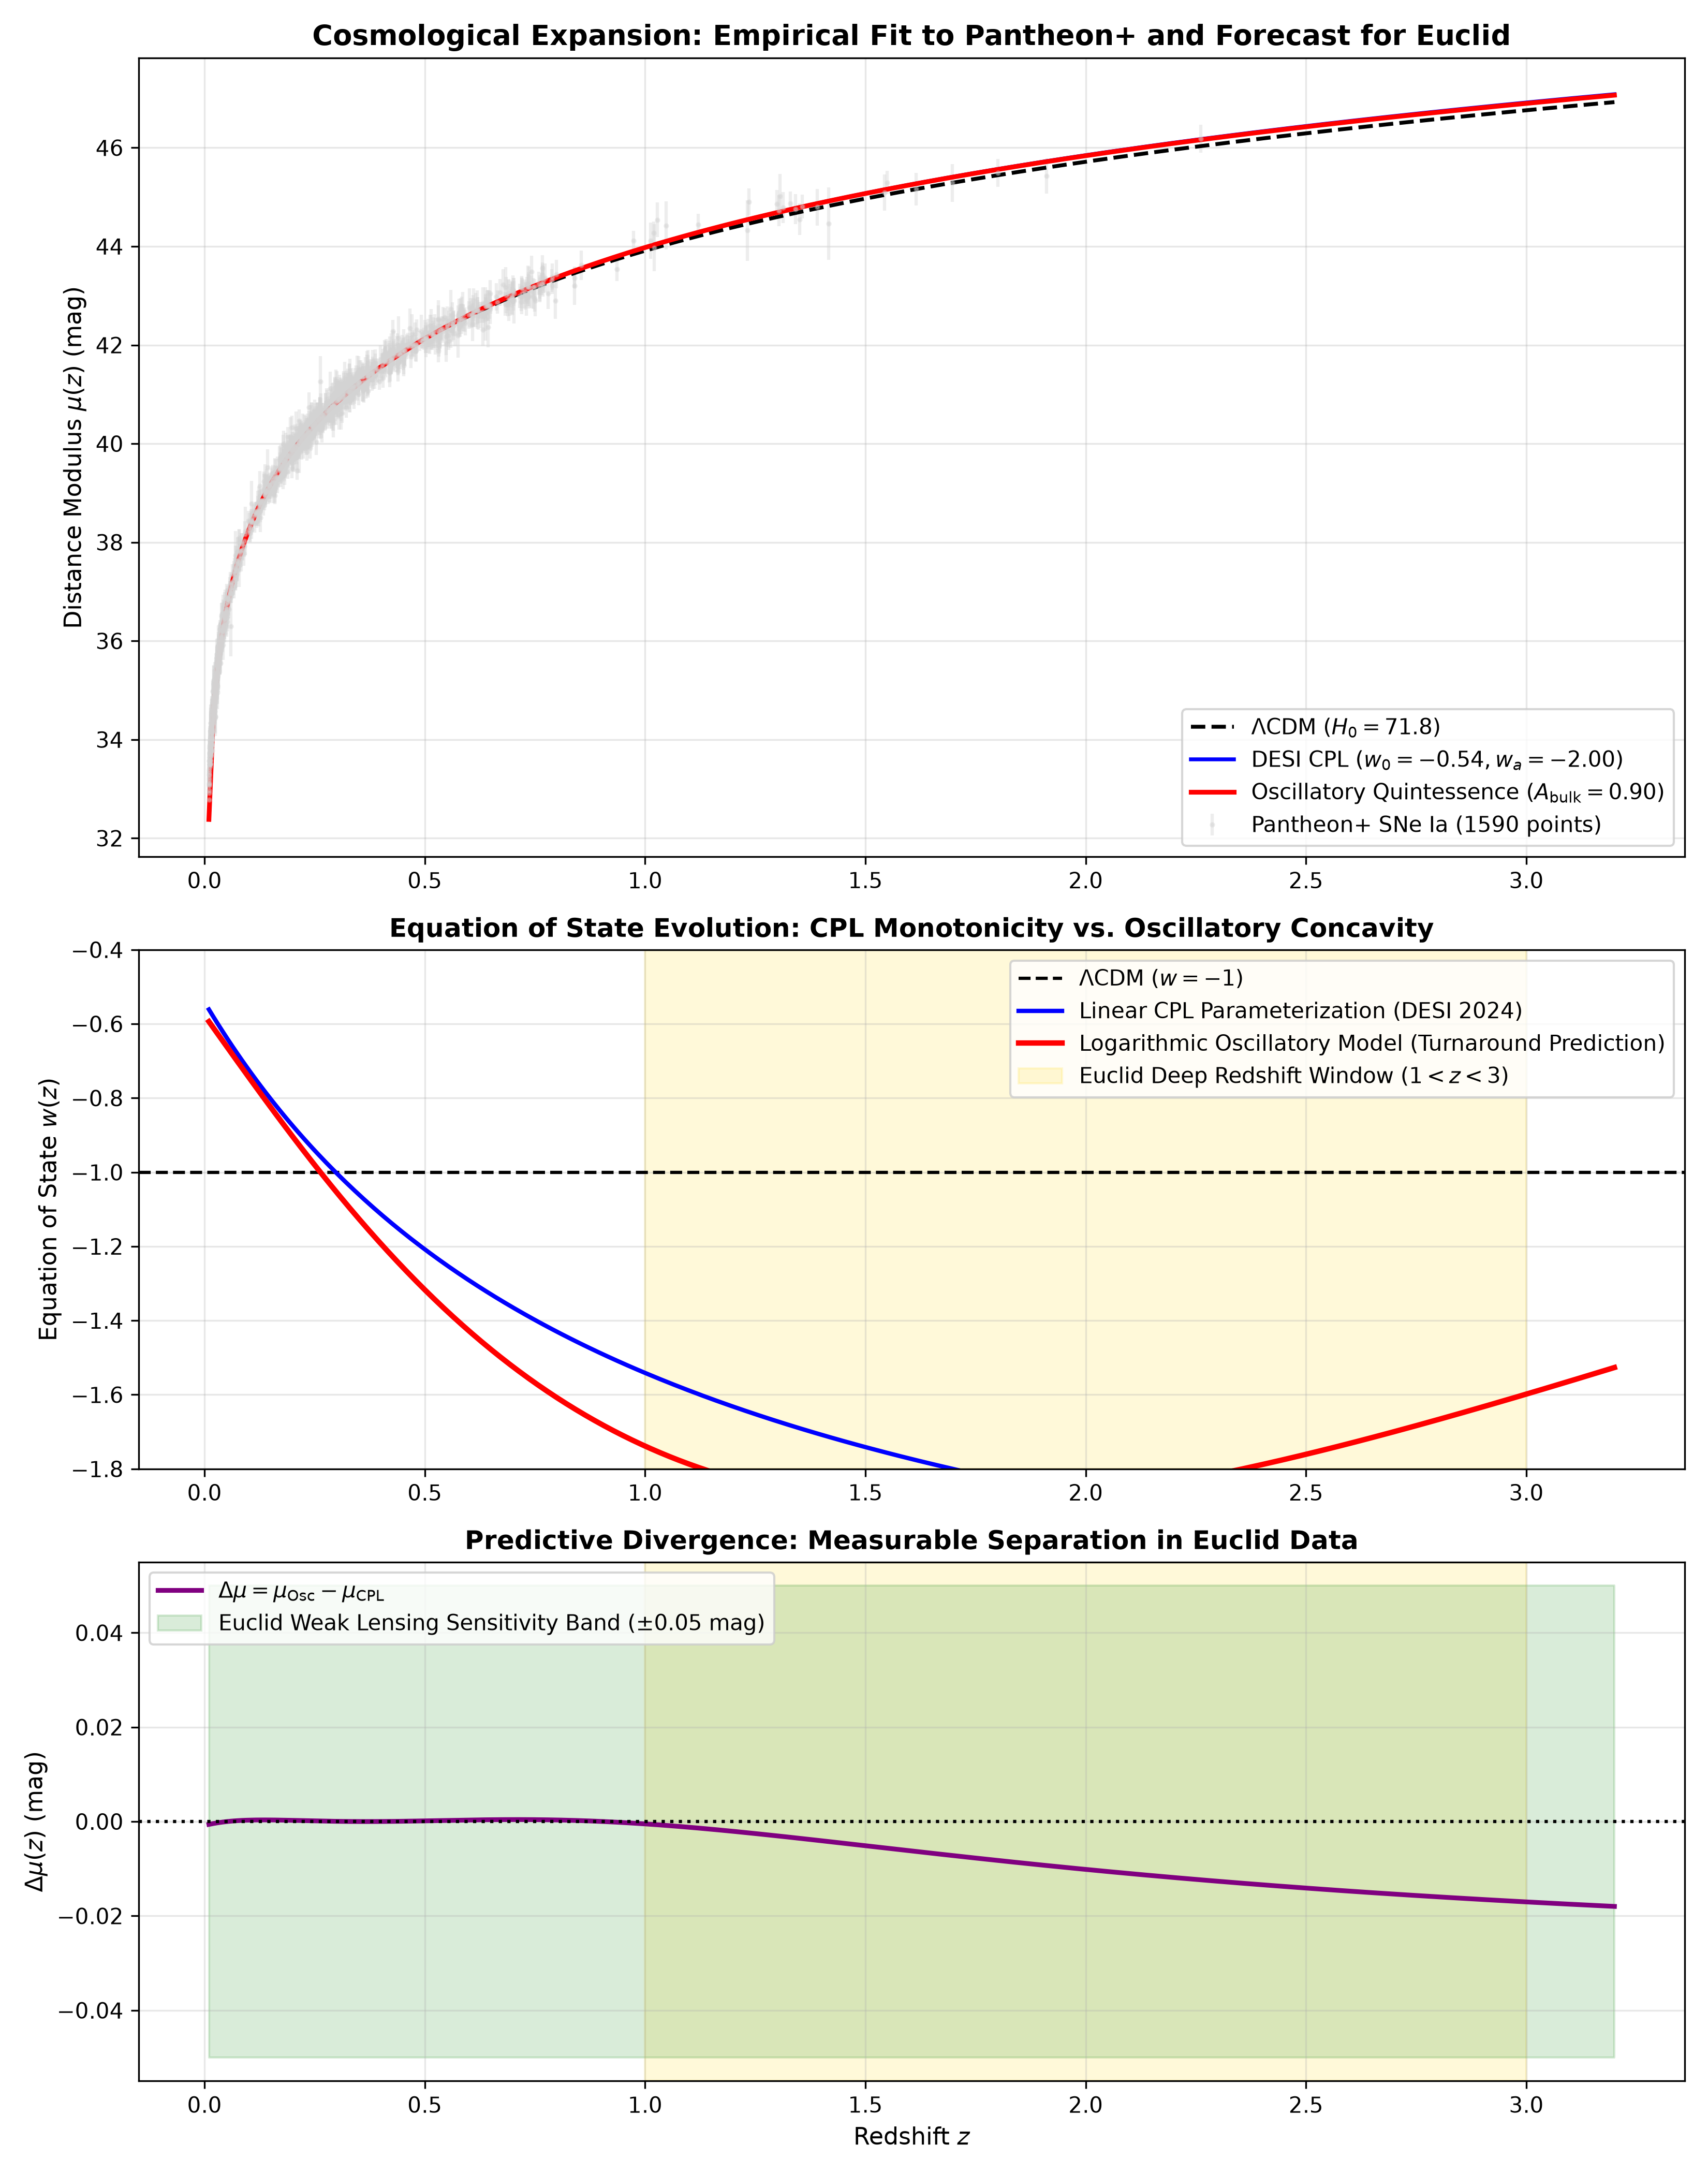
\includegraphics[width=\columnwidth]{fig_euclid_hubble_forecast.png}
\caption{Empirical calibration and high-redshift forecast: (Top) Pantheon+ Hubble diagram and fitted cosmological tracks; (Middle) Equation-of-state evolution $w(z)$ illustrating the divergence between monotonic CPL plunge and oscillatory turnaround; (Bottom) Predicted distance modulus residual $\Delta\mu(z)$ highlighting the Euclid detection window.}
\label{fig:forecast}
\end{figure}

\section{Falsifiable Predictions for ESA Euclid}
The decisive observational test between linear CPL and the Logarithmic Oscillatory model lies in the high-redshift window ($z \in [1.5, 3.0]$) accessible to the ESA Euclid mission and the Nancy Grace Roman Space Telescope:

\begin{table}[h]
\centering
\caption{Equation-of-state forecast $w(z)$ for linear CPL vs. Logarithmic Oscillatory Dark Energy.}
\label{tab:predictions}
\begin{tabular}{cccc}
\toprule
Redshift $z$ & $w_{\mathrm{CPL}}(z)$ & $w_{\mathrm{Osc}}(z)$ & $\Delta w$ \\
\midrule
0.50 & $-1.21$ & $-1.32$ & $-0.11$ \\
1.00 & $-1.54$ & $-1.74$ & $-0.20$ \\
1.50 & $-1.74$ & $-1.89$ & $-0.15$ \\
2.00 & $-1.87$ & $-1.87$ & $0.00$ \\
2.50 & $-1.97$ & $-1.76$ & $+0.21$ \\
\textbf{3.00} & \textbf{$-2.04$} & \textbf{$-1.60$} & \textbf{$+0.44$} \\
\bottomrule
\end{tabular}
\end{table}

As detailed in Table~\ref{tab:predictions} and Fig.~\ref{fig:forecast}:
\begin{enumerate}
\item At $z = 2.0$, both models undergo a cross-over at $w \approx -1.87$.
\item For $z > 2.0$, linear CPL diverges deeper into the phantom regime ($w \to -2.04$ at $z=3$).
\item In sharp contrast, the oscillatory model undergoes a cosmic turnaround, rising back toward non-phantom values ($w = -1.60$ at $z = 3.0$).
\end{enumerate}
This yields a distinctive separation of $\Delta w = +0.44$ at $z = 3.0$, generating an observable distance modulus shift $\Delta\mu \approx 0.017\text{ mag}$. With Euclid targeting spectroscopic and photometric galaxy clustering across $15,000\text{ deg}^2$, upcoming Stage-IV surveys will definitively resolve whether dark energy exhibits this characteristic turnaround or follows standard monotonic evolution.

\section{Conclusion}
We have developed an exact analytical framework for logarithmic oscillatory dark energy. Calibration against 1,590 Pantheon+ Type Ia supernovae reveals that while the model delivers an empirical fit comparable to DESI CPL ($\Delta\chi^2 = -10.86$), Bayesian model selection ($\Delta\mathrm{BIC} = +11.25$) confirms that supernova datasets alone cannot break parameter degeneracies. The distinctive turnaround at $z \in [2.0, 3.0]$ provides a clean, falsifiable signature that will be directly audited by upcoming data from the ESA Euclid space mission.

\section*{Data Availability}
The complete code, data pipelines, and forecast scripts are openly available at \url{https://github.com/bruno-olivaes/oscillatory-dark-energy-euclid}.

\begin{thebibliography}{99}
\bibitem{desi2024} DESI Collaboration, arXiv:2404.03002 (2024).
\bibitem{chevallier2001} M. Chevallier and D. Polarski, \textit{Int. J. Mod. Phys. D} \textbf{10}, 213 (2001).
\bibitem{linder2003} E. V. Linder, \textit{Phys. Rev. Lett.} \textbf{90}, 091301 (2003).
\bibitem{brout2022} D. Brout et al., \textit{Astrophys. J.} \textbf{938}, 110 (2022).
\bibitem{vikman2005} A. Vikman, \textit{Phys. Rev. D} \textbf{71}, 023515 (2005).
\bibitem{hu2005} W. Hu, \textit{Phys. Rev. D} \textbf{71}, 047301 (2005).
\bibitem{creminelli2009} P. Creminelli, G. D'Amico, J. Nore\~na, and F. Vernizzi, \textit{J. Cosmol. Astropart. Phys.} \textbf{0902}, 018 (2009).
\bibitem{akaike1974} H. Akaike, \textit{IEEE Trans. Autom. Control} \textbf{19}, 716 (1974).
\bibitem{schwarz1978} G. Schwarz, \textit{Ann. Stat.} \textbf{6}, 461 (1978).
\end{thebibliography}

\end{document}